\chapter{}

\section{The QCD Lagrangian}

In studying a system where only strong interactions are relevant, one turns to the QCD Lagrangian. It is a functional of the quark fields, $\psi$, which are 4-component Dirac spinors, and of the gluon fields, $A^a_\mu$, which are real-valued four-vectors; both are functions of spacetime. For a theory with $N_c$ colors, considering a single flavor of quarks with mass $m$,
% in the presence of external color charge sources $J^\mu (x)$,
the Lagrangian is
\begin{equation}
	\mathcal{L}_\text{QCD} = \overline{\psi} \left(i \gamma^\mu D_\mu - m \right) \psi - \frac{1}{2} \Tr_c \left[ F_{\mu \nu} F^{\mu \nu} \right] %\textcolor{blue}{-2 \Tr [A_\mu J^\mu]}
	\label{eq:QCD_Lagrangian}
\end{equation}
where $D_\mu$, the covariant derivative, is given by:
\begin{equation}
	D_\mu =  \partial_\mu - i g A_\mu, \quad \text{where }  A_\mu = A_\mu^a T_a
\end{equation}
and $F^{\mu \nu}$, the gluon field strength tensor, is given by:
\begin{equation}
	\begin{split}
		F_{\mu \nu} & = \partial_\mu A_\nu - \partial_\nu A_\mu - ig [A_\mu, A_\nu] \equiv F_{\mu \nu}^a T_a\\
		F_{\mu \nu}^a & = \partial_\mu A_\nu^a - \partial_\nu A_\mu^a + g f^{a b c} A^b_\mu A^c_\nu
	\end{split}
\end{equation}
%\textcolor{blue}{and $J_\mu$, similarly to $A_\mu$, is a four-vector and  a linear combination of the $T_a$:
%\begin{equation}
%	J_\mu \equiv J_\mu^a T^a
%\end{equation}}
$g$ is the Strong Force's coupling constant; $T^a$ are the SU($N_c$) generators in the fundamental representation\footnote{Normalized such that $\Tr_c [T^a, T^b] = \delta^{ab}/2$}, and $f^{abc}$ are the SU($N_c$) structure constants; $\Tr_c$ denotes a color-trace, that is, a trace in color space, the space of the $T_a$ matrices' indices; and $\overline{\psi}$ is the quark field's Dirac adjoint, equal to $ \psi^\dagger \gamma^0$.

%where the 4-component Dirac spinor $\psi$ is the quark field, a function of spacetime; $\overline{\psi}$ is its Dirac adjoint, $ \psi^\dagger \gamma^0$; $m$ is that quark flavour's mass; $D^\mu$ is the covariant derivative, obtained from the four-vector $A^\mu$, which is in turn obtained from a linear combination of the SU($N_c$) generators in the fundamental representation, $T^a$, with the real-valued gluon fields $A_\mu^a$, functions of spacetime, serving as coefficients; $F^{\mu \nu}$ is called the gluon field strength tensor; and $\Tr_c$ denotes a color-trace, that is, a trace in color space, where the $T_a$ live.

Writing the Lagrangian with all indices explicit,
\begin{equation}
	\mathcal{L}_{\text{QCD}} = \left(\psi_\alpha^i \right)^*  \left( \gamma^0  \right)_{\alpha \beta} \left(i \left(\gamma^\mu \right)_{\beta \gamma} \left( \delta^{ij} \partial_\mu - i g A^a_\mu \left( T^a \right)^{ij} \right) - \delta_{\beta \gamma} \delta^{ij} m \right) \psi_\gamma^j - \frac{1}{4} F_{\mu \nu}^a F^{\mu \nu}_a
	%\textcolor{blue}{- A_\mu^a J^\mu_a}
	\label{eq:QCD_Lagrangian_Indices}
\end{equation}
where $\alpha, \beta, \gamma = 1,2,3,4$ are Dirac indices, $i,j=1, ..., N_c$ are color indices in the fundamental representation, $a = 1, ..., {N_c}^2-1$ are color indices in the adjoint representation, and $\mu,\nu = 0,1,2,3$ are spacetime indices when using Minkowski coordinates.

To obtain the Lagrangian considering all flavors of quarks, one need only add copies of the first term of Eq. (\ref{eq:QCD_Lagrangian}) for each quark flavor's quark fields.

Given the presented QCD Lagrangian, the corresponding Euler-Lagrange equations relating to the gluon fields $A$ are called the Yang-Mills equations, which can be thought of as the QCD equivalent to Classical Electrodynamics' Maxwell's equations.
%In the absence of color sources,\footnote{That is, in the absence of source terms in the Lagrangian and taking the usual color current, $g \overline{\psi} \gamma^v \psi$, to be $0$.}
In the absence of quark fields ($\psi=0$), they read:
\begin{equation}
	[D_\mu, F^{\mu \nu}] = 0
	%\textcolor{blue}{J^\nu}
	\label{eq:homogenous_Yang-Mills}
\end{equation}
%g \overline{\psi} \gamma^v \psi +

\section{[A picture of nuclear matter]}
\label{sec:nuclear_matter}

\textcolor{red}{[Part of it may migrate. At some point before, introduce the proton as something more than 3 quarks]}

Probing hadrons at high energies in scattering experiments has allowed exploring the interior structure of nucleons. Data from  both fixed-target and collider (HERA, Tevatron, LHC) experiments has been compiled in order to obtain pictures of the parton content of hadrons.

At HERA, electrons (or positrons) and protons were accelerated to collide at center of mass energies of around $\sqrt{s} = \qty{300}{GeV}$. In some of these collisions, the momentum transfer $Q^\mu$ from the electron to the proton via a virtual photon was large enough ($Q^2 > \qty{200}{GeV^2}$) to disintegrate the proton into a shower of hadrons $(e  + p \to e + X)$; these are called \gls{DIS} collisions, whose cross-sections are valuable in unveiling the proton's parton content. The greater the virtual photon's energy, the greater its ability to resolve structures of smaller scale than the proton radius and with shorter characteristic timescales. \gls{DIS} collisions have also been studied for this purpose using muons, $\mu$, and neutrinos, $\nu$, as probes, and neutrons as targets. At the Tevatron and LHC colliders, data from $p\overline{p}$ and $pp$ collisions, respectively, has contributed to the study of the gluon content of protons, specifically. \cite{Thomson8:2013}\cite{PDG_2024}

The contributions from these many experiments have permitted the measurement of the proton's \glspl{PDF}, which quantitatively characterize the parton content of a hadron. They translate the abundance, inside the proton, of a given parton species carrying a certain fraction of its momentum (in a frame of reference where the proton's momentum is large). The \gls{PDF} of a species of parton $q$ inside the proton, $q(x)$, is defined such that the number of $q$ partons carrying a fraction of the proton's momentum between $x$ and $x + \Delta x$ is given by $q(x)\Delta x$. These functions actually also depend on the energy scale of the process used to probe the proton, $Q^2$, since a greater exchange of energy allows probing finer features of the proton, increasing its \glspl{PDF} at small $x$, for example. \cite{Thomson8:2013}

Fig. \ref{fig:PDFs} shows the different parton species' \glspl{PDF} for the proton. For $0.1 \lesssim x < 1$, the ``valence" quarks $u$ ($\mathbf{u}_V$)and $d$ ($\mathbf{d}_V$) dominate -- in the relative proportion expected from the static quark model for the proton, $uud$. However, for $x \lesssim 0.02$, they are overtaken by a ``sea" of quarks and antiquarks ($\overline{\mathbf{u}}$, $\overline{\mathbf{d}}$, $\mathbf{s}$, $\mathbf{c}$, $\mathbf{b}$), which, for the same flavor, have identical \glspl{PDF}. For small $x$, however, the most abundant parton is, by far, the gluon ($\mathbf{g}$).

\begin{figure}\centering
	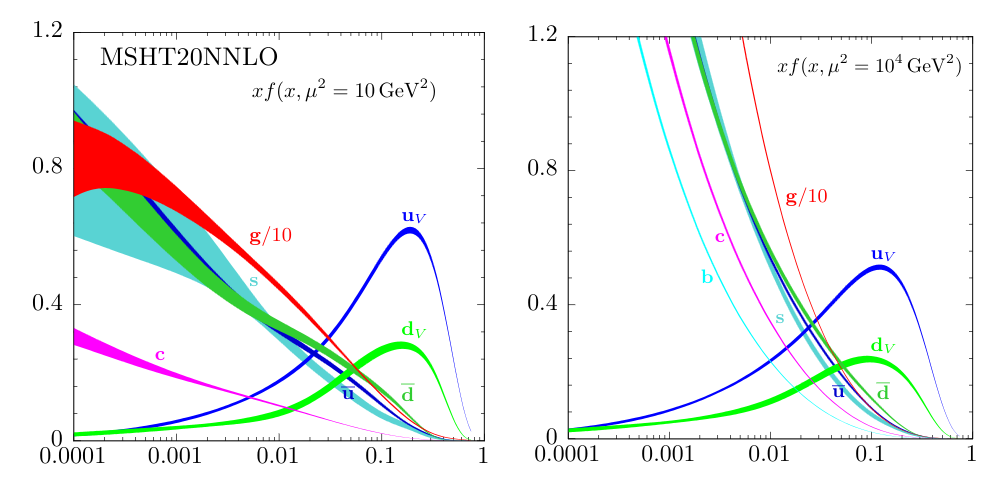
\includegraphics[width=\textwidth]{figures/external/PDFs_2021.png}
	\caption{The proton's \glspl{PDF} multiplied by $x$ for the case of unpolarized beams at the energy scales $\mu^2 = \qty{10}{GeV^2}$ (left) and $\mu^2 = 10^4\qty{}{GeV^2}$ (right). The gluon's \gls{PDF} appears scaled down by a factor of 10. \cite{PDG_2024} Originally from and calculated by the MSHT Group. \cite{Bailey_2021}}
\label{fig:PDFs}\end{figure}

\section{Gluon Saturation}
\label{sec:gluon_saturation}

%\textcolor{red}{[Refer previous discussion of low-$x$ gluon abundance]}

This dominance of the gluon ``sea" at low-$x$ is predicted by \gls{QCD}, as discussed here regarding the splitting function of the gluon and the \gls{BFKL} equations.
%since the fits that obtain fid 1's pdfs include the DGLAP (and BFKL?) equations, this feels a bit dishonest, maybe?

The splitting function of non-Abelian gauge bosons such as the gluon is a well know \gls{QCD} result. It returns the probability of emission by a parton of a gluon with relative transverse momentum $\mathbf{k}_\perp$ and a fraction $x$ of its longitudinal momentum. At lowest order in $\alpha_S$ and for small $x$, it reads \cite{Albacete_2014,Gelis_2010}:

\begin{equation}
	\diff P \propto \frac{\alpha_S}{\pi^2} \frac{\diff^2 \mathbf{k}_\perp}{\textcolor{blue}{k_\perp}} \frac{\diff x}{x}
\end{equation}
the singularity of this probability as $x \to 0$ suggests a picture of abundance of small-$x$ gluons within all hadrons, which grows uncapped as partons emit small-$x$ gluons, which themselves emit smaller-$x$ gluons or produce quark-antiquark pairs which also serve as gluon emitters. However, gluon densities may not explode as $x \to 0$, as unitarity would be violated. \cite{Albacete_2014}

Below a certain value of $x$, non-linear dynamics not considered so far should take over and tame the divergence, \textit{saturating} the low-$x$ gluon density in the hadron. The onset of saturation is controlled by the saturation scale, $Q_s(x)$, a transverse momentum scale below which non-linear effects become relevant. \cite{Albacete_2014}

One interpretation of these non-linear effects is the onset, above certain gluon densities, of gluon recombination. Above that threshold, the probability of emission of a new gluon becomes comparable to the probability of recombination of gluons, stopping the growth of their density (Fig. \ref{fig:gluon_recombination}).

\begin{figure}\centering
	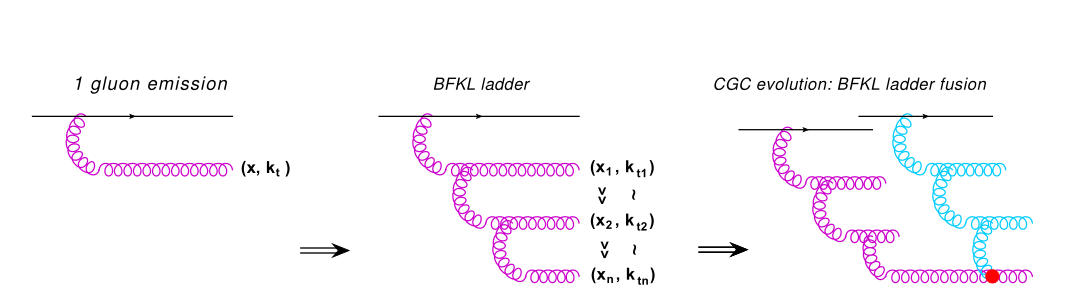
\includegraphics[width=\textwidth]{figures/external/gluon_recombination.png}
	\caption{The onset of gluon recombination. Above a certain gluon density, gluon recombination (red dot) becomes comparatively likely to gluon emission (the pink and blue ladders of gluons). Taken from \cite{Albacete_2014}.}
\label{fig:gluon_recombination}\end{figure}

More formally, the \gls{BFKL} \gls{QCD} evolution equation is a linear differential equation that governs how gluon density in momentum space within a hadron should evolve with $x$ when that hadron is probed at a certain energy scale. It is a linear equation, and it predicts
%an exponential growth of the gluon density with rapidity, Y = ln(1/x); equivalently, it predicts
a divergence of the gluon density as $x \to 0$. The equation does not contain terms reflecting interference between emitters of gluons, as it assumes the hadron to be a dilute parton system. However, making the probability of emission of a new gluon dependent on the present gluon density allows for saturation to be reached when gluon generation and gluon recombination balance out. QCD evolution equations which attempt to incorporate this effect have additional, non-linear, density-dependent terms, such as the \gls{GRL-MQ} equation. \cite{Albacete_2014}

\section{The Color Glass Condensate and The McLarran-Venugopalan Model}
\textcolor{purple}{Should I start with describing protons with the CGC and say it's the same for the nuclei? or should I start right away using the word nucleus?}

%\textcolor{blue}{[Separation between the CGC and the MV model]}

The \gls{CGC} is an effective theory of \gls{QCD} for high-energy \gls{QCD} scattering applied to allow the description of the aforementioned saturated gluons \cite{Gelis_2010}, which evade standard perturbation techniques. It is one of the approaches used to study initial state effects in \glspl{HIC} and has stood out due to its practical applicability and phenomenological success.\cite{Albacete_2014} It hinges on the partition of the parton content of a hadron, in the \gls{IMF},
%-- in this case, a heavy nucleus --
via approximations, into static color charges and the dynamic classical gluon fields, representing the saturated gluons, which they generate via the processes described in Section \ref{sec:gluon_saturation}.\cite{Gelis_2010} In this case, the hadron in question is a heavy nucleus, which is made up of neutrons and protons whose contents are previously discussed.
%The \gls{CGC} effective theory of \gls{QCD} for high-energy \gls{QCD} scattering is one of the approaches used to study initial state effects in \glspl{HIC}, and has stood out due to its practical applicability and phenomenological success. \cite{Albacete_2014}

%\textcolor{purple}{- Separation of the contents of the nucleus//hadron according to their momentum. This is done in the INFINITE MOMENTUM FRAME.}

\subsection{Classical saturated gluon fields}
\textcolor{purple}{YET UNJUSTIFIED: why $N \sim 1/g^2$; why $g$ is small; do the creation operators create a gluon with a specific momentum $(x,\mathbf{k}_\perp)$?}

Starting by justifying the treatment of the saturated gluons as classical fields, the saturated gluon densities at low-$x$ discussed previously in Sections \ref{sec:nuclear_matter} and \ref{sec:gluon_saturation} imply gluon (or color) fields of the order $A \sim 1/g$, which does not allow their treatment through standard perturbative techniques\footnote{For example, in calculating the matrix element $\mathcal{M}$ for a \gls{QCD} process using a series expansion in powers of $g$, all terms are proportional to $gA \sim \mathcal{O}(1)$, which does not allow truncating the series in order to estimate $\mathcal{M}$ -- all orders need to be summed.}.\cite{Albacete_2014} However, it opens the possibility of their treatment as classical fields.

Comparing the occupation number of the saturated gluon fields and the commutator of their creation, $a^\dagger$, and annihilation, $a$, operators, \cite{Albacete_2014}
\begin{equation}
	N = a^\dagger a \sim \frac{1}{g^2} \quad \gg \quad [a^\dagger, a] \sim 1
\end{equation}
it is possible to state that quantum corrections to the classical solution, where the fields commute, are negligible. Thus, it is reasonable to treat the low-$x$ gluon fields as classical fields.

\subsection{Partition of the nucleus's parton content} \label{sec:scale_separation}

In order to illustrate the partition of the parton content of the nucleus into a static and a dynamic part, it is necessary to move to the infinite momentum frame. In the \gls{IMF}, the nucleus is boosted along its direction of motion so as to make the momenta of its constituent partons approximately collinear to its own. In this frame, considering a nucleus moving in the positive $x^1$ direction with large total longitudinal momentum $P$ much greater than its mass, $m_A$, the four-momenta of the nucleus and of one of its constituent partons in Minkowski coordinates are: \cite{Thomson8:2013}
\begin{subequations}
	\label{eq:IMF}
	\begin{align}
		\text{Nucleus: } & P^\mu = (P,P,0,0)
		&
		\text{Parton $i$: } & p^\mu = (x_i P, x_i P, \sim 0, \sim 0)
		\\
		\intertext{
			where $0<x_i<1$ is the fraction of the nuclear longitudinal momentum carried by the $i$-th parton; it was further assumed that the boost applied was such that $x_i P \gg m_i$, with $m_i$ being the $i$-th parton's mass. In light-cone coordinates (Appendix \ref{ap:Light_Cone}),}
		\text{Nucleus: } & P^\mu = (P^+,0,0,0)
		&
		\text{Parton $i$: } & p^\mu = (x_i P^+, \sim 0, \sim 0, \sim 0)
	\end{align}
\end{subequations}
where $P^+ = \sqrt{2} P$. It becomes clear that $x_i$ is also the $i$-th parton's fraction of the nuclear light-cone $+$-momentum.

%\textcolor{red}{- Problem: not all of the boosted partons will obey $p_i^2 \gg m_i^2$ right? or even $p^1 \gg p_T$}

The uncertainty principle can be used to evaluate the approximate extent of each parton over the $x^-$ and $x^+$ coordinates: \cite{Lappi_notes,Albacete_2014}
\begin{subequations} \label{eq:Uncertainty_Relations}
	\begin{gather}
		\Delta x^- \propto \frac{1}{p^+} = \frac{1}{x_i P^+} \\
		\Delta x^+ \propto \frac{1}{p^-} = \frac{2p^+}{(p^0)^2 - (p^1)^2} = \frac{2p^+}{(\mathbf{p}_\perp)^2 + {m_i}^2} \approx \frac{2 x_i P^+}{(\mathbf{p}_\perp)^2}
	\end{gather}
\end{subequations}
where $\mathbf{p}_\perp$ is the $i$-th parton's transverse momentum, which was taken to be negligible in Eqs. (\ref{eq:IMF}) when compared to its longitudinal momentum.

Two useful conclusions about the $x^+,x^-$  scales of high-$x$ and low-$x$ partons may be extracted from the uncertainty relations:
\begin{itemize}
	\item[1)] high-$x$ partons are highly localized in the $x^-$ direction. That is, they occupy a very thin ``slice" of space in the $x^-$ direction.
	\item[2)] high-$x$ partons are more delocalized in the $x^+$ direction than their low-$x$ counterparts. That is, their typical $x^+$ scale %\textcolor{red}{(often called light-cone time -- introduce $x^+/t$ equivalence somewhere??)}
		is greater than the low-$x$ partons'. Equivalently, the fluctuations of the low-$x$ parton fields are much shorter along the $x^+$ direction than for the high-$x$ parton fields.
\end{itemize}

\textcolor{purple}{? Include the naive \cite{Lappi_notes} interpretations? 1) the Lorentz-contraction of the nucleus along $x^1$. 2) Time dilation experienced by valence partons.}

It is from the second point that a hierarchy arises, central to the \gls{CGC} formalism, of partons separated according to their $x$-values. A $+$-momentum scale, $\Lambda^+$, is introduced to separate the high-$x$, or valence, partons and the low-$x$ partons. From the perspective of the latter, the first have very slow dynamics\textcolor{red}{ \footnote{\textcolor{blue}{Also slow in the timescale of the pre-hydrodynamic stage?}}} in $x^+$; in the limit of this argument, they are \emph{static} in $x^+$; for particles traveling at the speed of light, being static in $x^+$ is equivalent to being static in $t$. As such, in the \gls{CGC}, valence partons become constant color charges, which serve as sources for the \emph{dynamic} low-$x$ parton fields.
% Regarding the low-$x$ partons,
As was introduced in sections \ref{sec:nuclear_matter} and \ref{sec:gluon_saturation}, the partonic content of protons, and hence of the nucleus, is dominated by gluons at low-$x$. Therefore, the dynamic fields are taken to be gluon, also called color, fields.

%Regarding the low-$x$ partons, they are, in contrast, dynamic. Additionally since the partonic content of protons, \textcolor{blue}{ and hence of the nucleus}, is dominated by gluons at low-$x$, as introduced in sections \ref{sec:nuclear_matter} and \ref{sec:gluon_saturation}, these dynamic fields are taken to be gluonic fields, also called color fields.

The parton content of the nucleus is thus divided into the group of high $+$-momentum ($p^+ > \Lambda^+$) static color charges and the group of low $+$-momentum ($p^+ < \Lambda^+$) dynamic classical gluon fields which they generate. The static color charges may themselves be treated as classical \cite{Albacete_2014,McLerran_1994_classic_source}
and are eikonally coupled to the classical gluon fields; that is, they suffer negligible recoil from their interactions with the color fields, when compared to their longitudinal momentum.\cite{Gelis_2010} Thus, they are introduced into the \gls{QCD} Lagrangian (Eq. (\ref{eq:QCD_Lagrangian_Indices})) as classical color current 4-vectors in the term $A_\mu^a J^\mu_a$. Since, now, the formalism does not include quantum quark fields, Eqs. \ref{eq:QCD_Lagrangian} and \ref{eq:QCD_Lagrangian_Indices} become, respectively,%\textcolor{red}{the absence of dynamic color fields gets rid of the first term. The influence of the static color sources on the system is brought back via the} addition of an external color source term to the \gls{QCD} Lagrangian. Equations \ref{eq:QCD_Lagrangian} and \ref{eq:QCD_Lagrangian_Indices} become, respectively,
\begin{align}
	\mathcal{L}_\text{QCD}' & = - \frac{1}{2} \Tr_c \left[ F_{\mu \nu} F^{\mu \nu} \right] + 2 \Tr_c [A_\mu J^\mu] \\
	\mathcal{L}_\text{QCD}' & =  - \frac{1}{4} F_{\mu \nu}^a F^{\mu \nu}_a + A_\mu^a J^\mu_a
\end{align}
where $J^\mu \equiv J^\mu_a T^a$.

Consequently, the corresponding Euler-Lagrange equations for the gluon fields $A$ become:
\begin{equation}
	[D_\mu, F^{\mu \nu}] = J^\nu
\end{equation}
which, provided an expression for the external color currents, may be solved for the classical gluon fields.

Seeing $J^\mu$ as a classical color current describing the high-$x$ partons, which travel at near the speed of light in the $x^1$ direction, then, in light-cone coordinates, its only non-vanishing component is $J^+$ (Eq. (\ref{eq:Nonvanishing_current_+})). Additionally, it will directly depend on the number color charge distribution of the valence partons, $\rho (x) \equiv \rho_a(x) T^a$ (Eq. (\ref{eq:J_from_rho})).
\begin{gather}
	J^\mu = \delta^\mu_+ J^+ \label{eq:Nonvanishing_current_+} \\
	J^+ = g \rho (x^\mu) \label{eq:J_from_rho}
\end{gather}

From the previous discussion on the static nature of the color charges, $\rho$'s dependence on $x^+$ can be dropped. Furthermore, due to the first conclusion drawn from the uncertainty relations (Eqs. \ref{eq:Uncertainty_Relations}), the color charge distribution function describing the placement of the static valence partons is very thin in the $x^-$ direction. In the limit where this thin $x^-$ dependence factorizes to a Dirac-delta function, the valence color current four-vector is, in light-cone coordinates:
\begin{equation}
	{J}^\mu = (g \delta (x^-) \rho (\mathbf{x}_\perp), \sim 0, \sim 0, \sim 0)
	\label{eq:+_Current}
\end{equation}
where the charge distribution has been taken to be longitudinally homogenous and $\rho$ has become an area number charge density.

\subsection{The stochastic nature of $\rho$}
The color charge distribution $\rho$, from which $J^\mu$ and, consequently, the evolution of the gluon fields are obtained, is fixed for a single nucleus in a single event. It is different, however, for different nuclei and for each event, constituting a stochastic variable \cite{Gelis_2010} which isn't experimentally accessible.  Even for the same nucleus, $\rho$ would change if enough time is allowed to pass in order for the nucleus to travel over a $x^+$ greater than the valence partons' typical $x^+$ scale \cite{Gelis_Habilitation}. In order to calculate an observable $\mathcal{O}$ out of many events within the \gls{CGC} effective theory, one must determine its average value considering all the different possible color charge distributions and their probabilities: \cite{Gelis_2010}
\begin{equation}
	\left< \mathcal{O} \right> = \int [\diff \rho] W[\rho] \mathcal{O}[\rho]
\end{equation}
where $\mathcal{O}[\rho]$ is the observable's value for the particular charge distribution $\rho$, and $W[\rho]$ is a functional probability distribution evaluated for that same charge distribution, describing its probability of occurring.

\subsection{Quantum Corrections and the McLerran-Venugopalan Model}

So far, the effect of the choice of a $+$-momentum scale $\Lambda^+$ to separate low- and high-$x$ partons on the final result of an observable, $\left< \mathcal{O} \right>$, has been neglected. Indeed, once a $+$-momentum scale has been set, one neglects that certain low-$x$ partons sorted into the category of classical gluon fields actually behave as static color charges for lower-$x$-still partons\footnote{In the language of Section \ref{sec:gluon_saturation}, even a low-$x$ gluon can serve as an emitter of lower-$x$ gluons.} \cite{Albacete_2014}. Thus, choosing a different $\Lambda^+$ would lead to different observable values. When changing the value of the $+$-momentum scale from $\Lambda^+$ to ${\Lambda^+}'$, it is possible, however, to renormalize $\rho$, correlators of different $\rho$ or the functional probability distribution  $W$ in order to incorporate those quantum corrections into the \gls{CGC} effective theory and preserve the value of the observables, making them independent of $\Lambda^+$, while keeping the calculation procedure strictly classical \cite{Albacete_2014}. Choosing to incorporate these quantum corrections into the probability distribution, which then becomes dependent on the $+$-momentum scale, $W_{\Lambda^+}$, its evolution with $\Lambda^+$ is ruled by a functional \gls{JIMWLK} equation \cite{Gelis_2010}. Other methods to incorporate quantum corrections into the effective theory exist, as well as variations on the \gls{JIMWLK} equation \cite{Albacete_2014}.

In spite of this achievement, an initial probability function $W_{\Lambda^+_0}$ is still necessary before studying its evolution with the $+$-momentum scale; this function can be seen as an initial condition for the \gls{JIMWLK} equation. The \gls{MV} model provides that initial condition, for the case of large nuclei. It is physically motivated and may even be used directly, without needing to be evolved into $x$-scales much smaller than $\Lambda_0^+$, for the study of $pA$ or $AA$ collisions where the values of $x$ are not small enough to require that evolution. \cite{Gelis_2010}  $W_{\text{MV}}$, not normalized, is given by \cite{Gelis_Habilitation}:
\begin{equation}
	W[\rho_\text{\textcolor{blue}{$a$}}] = \exp \left[ - \int \diff^2 \mathbf{x}_\perp \frac{\rho_a(\mathbf{x_\perp})\rho_a(\mathbf{x_\perp})}{2 \mu^2} \right]
\end{equation}
which has an associated charge density 2-point correlator:
\begin{equation}
	\left< \rho_a(\mathbf{x}_\perp) \rho_b (\mathbf{y}_\perp) \right> = \mu^2 \delta_{ab} \delta^2 (\mathbf{x}_\perp - \mathbf{y}_\perp)
\end{equation}

\textcolor{red}{How do I relate these two?}

\textcolor{blue}{[Some authors use $\mu(x^-)$, $\rho(x^-, \mathbf{x}_\perp)$ for $W$ \cite{Albacete_2014} or for the 2-point correlator \cite{Lappi_notes}. From what I saw, only \cite{Gelis_Habilitation} introduces the MV model without the $x^-$ coordinate here, but for $W[\rho_a]$ instead of $W[\rho]$.][Should I not factorize the $x^-$ as soon as I do, so that I can use those results here?]}

The \gls{MV} model's functional probability distribution $W_{MV}$ and corresponding charge density 2-point correlator are motivated physically for the case of large nuclei: \cite{Gelis_Habilitation}
\begin{itemize}
	\item[1)] Due to color confinement, color charge within different nucleons should be uncorrelated. Since charge densities at different transverse positions are associated with different nucleons/longitudinal superpositions of nucleons, they should also be uncorrelated.
	\item[2)] For large nuclei, at least at central positions, transverse color charge density results from the sum of many longitudinally aligned nucleons. Since the color charge of those nucleons is uncorrelated, then $\rho_\text{\textcolor{blue}{$a$}}(\mathbf{x}_\perp)$ is a sum of uncorrelated variables. Therefore, the Central Limit Theorem applies, and $\rho_\text{\textcolor{blue}{$a$}}(\mathbf{x}_\perp)$ should follow a Gaussian distribution.
\end{itemize}

%that constitute the classical color fields and the color charge sources

%\textcolor{blue}{[Talk about renormalization of the theory and the JIMWLK equations?] }

%\textcolor{red}{When to make the leap from the particle description of the mechanisms of parton creation/annihilation into classical fields.}

%- Description of the two classes of partons. Justified on Heisenberg uncertainty principle, delocalization in x- and x+ coordinates. Explain why only gluons in the lower class.

%Combining the separation of partons into static color charges and dynamic gluon fields with the classical treatment of those fields, \textcolor{red}{it is possible to study the system by solving the classical Yang-Mills equations (Eq. \ref{eq:Yang-Mills}) using Eq. \ref{eq:+_Current} as the external color current.}



%\textcolor{blue}{[Explanation of the classical low-$x$ gluon fields.]}


%\textcolor{purple}{The \gls{MV} model -- MODEL OF WHAT. INTRODUCED IN ... BY ... .}


%\textcolor{purple}{- Then the stochastic, Gaussian model for the static color charges (fuzzy)}

In this work, the non-evolved \gls{MV} model will be used. The application of this formalism to the two-nuclei system of a \gls{HIC} will be introduced over the next sections. It was first accomplished in \cite{Kovner_1995}.


\section{[Setting the stage/introducing the initial situation]}
In a HIC, \textcolor{red}{as previously introduced}, two heavy nuclei travel in opposite directions at near the speed of light before crashing into each other. For the purposes of this work, both nuclei will be taken to travel at the speed of light; because of this, they suffer length contraction along the direction of their trajectories, becoming infinitely thin/planar\footnote{\textcolor{red}{One reference makes a comparison between the longitudinal extent of the nucleus and the energy of the probe??}}. Furthermore, their collision is taken to be central, that is, the trajectories of their centers are perfectly aligned.

In the laboratory/center of mass frame, the $x^1$ axis is placed along the trajectories of the nuclei. The nucleus moving in the positive $x^1$ direction is identified as nucleus 1, and the one moving in the negative $x^1$ direction is identified as nucleus 2. The nuclei collide at $x^1 = 0$, at instant $t=0$. This system is invariant under boosts along the $x^1$ direction.

\begin{figure}\centering
	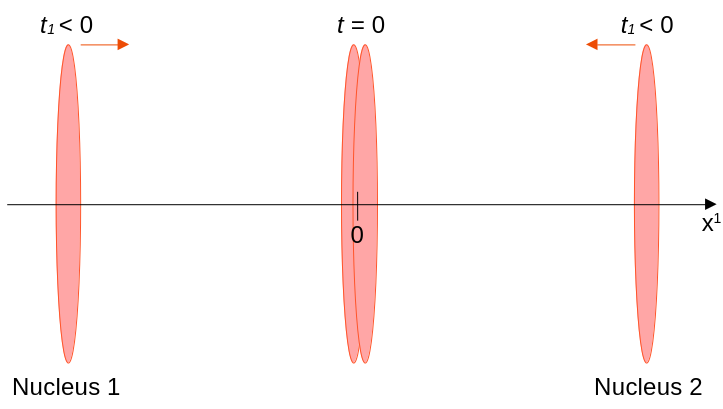
\includegraphics[width=0.7\textwidth]{figures/external/HIC.png}
	\caption{Two heavy nuclei, Lorentz-contracted into thin disks, travel along the $x^1$ axis in opposite directions until they collide at $t=0, x^1=0$.}
\label{fig:HIC}\end{figure}

As such, prior to the collision, each nucleus's position four-vector, $x^\mu = (x^0,x^1,x^2,x^3)$, in Minkowski coordinates, is:
\begin{equation*}
	\begin{split}
		\text{Nucleus 1}:& \quad (t,t,0,0) \\
		\text{Nucleus 2}:& \quad (t,-t,0,0)
	\end{split}
\end{equation*}

These trajectories are well-illustrated in the $x^1Ox^0$ plane:

\begin{figure}\centering
	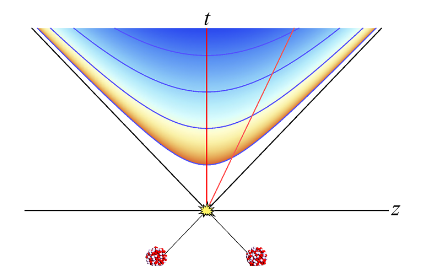
\includegraphics[width=0.7\textwidth]{figures/external/HIC_lightcone.png}
	\caption{A heavy-ion collision represented in the $x^1Ox^0$ plane. Both nuclei travel along the light-cone centered around the collision at coordinates $(0,0)$. Taken from \cite{vanderschee2014}.}
\label{fig:HIC_lightcone}\end{figure}

After the collision, the nuclei's approximately static high-$x$ partons, discussed in Section \ref{sec:scale_separation},
carry on in the direction they were moving at the speed of light, acting as color sources for the gluon fields then generated in the space between the now receding nuclei.
%\textcolor{red}{[They were already acting as color sources for fields, but in the other quadrants]}.
It is in this space that the pre-hydrodynamic stage to be studied is formed. Fig. \ref{fig:HIC_lightcone} already suggests the usefulness of the ligh-cone coordinate system (see Appendix \ref{ap:Light_Cone}), as the static color sources only travel along the edges of the light-cone centered on the collision coordinates $(0,0)$. In this coordinate system, the nuclei's position four-vectors, $x^\mu=(x^+,x^-,x^2,x^3)$, are:
\begin{equation*}
	\begin{split}
		\text{Nucleus 1}:& \quad (\sqrt{2}t,0,0,0) \\
		\text{Nucleus 2}:& \quad (0,\sqrt{2}t,0,0)
	\end{split}
\end{equation*}
and the collision coordinates remain at $(x^+=0,x^-=0)$.

In order to fulfill this work's objectives, it will be necessary to calculate the gluon fields generated in the space between the receding nuclei, making use of the classical Yang-Mills equations. The fields will be determined from the the static distributions of color charge of the receding nuclei.

\textcolor{red}{Next: event averages? Move the introduction to dEdx and $\hat{q}$ to before this? say they are the result of the color fields acting on the quark probe?}

\section{Solving The Yang-Mills Equations}

\subsection{One nucleus}
It is easiest to start by considering the case of a single nucleus, chosen to be Nucleus 1, moving in the positive $x^1$ direction. \textcolor{red}{First done in \cite{}, also done in \cite{} (good reference)}. The Yang-Mills equations are solved in the light-cone gauge, where $A^+=0$, an axial gauge condition. \textcolor{blue}{(\cite{Kovner_1995}: "one has direct access to the gluon distribution functions of the parton model")}

First of all, the external current inputted is checked to be consistent with the Yang-Mills equations; the current should be covariantly conserved:
\begin{equation}
	[D_\nu, J^\nu] = [D_\nu, [D_\mu, F^{\mu \nu}]] = 0
	\label{eq:covariant_conservation}
\end{equation}
\textcolor{blue}{ (proof should be left to an appendix?) where the second equality may be shown by use of the Jacobi Identity:
\begin{equation}
	\begin{split}
		& [D_\nu, [D_\mu, F^{\mu \nu}]] = - [D_\mu, [F^{\mu \nu}, D_\nu]] - [F^{\mu \nu}, [D_\nu, D_\mu]] \\
		%	\Leftrightarrow ~ & [D_\nu, [D_\mu, F^{\mu \nu}]] = - [D_\nu, [F^{\nu \mu}, D_\mu]] - [F^{\mu \nu}, [D_\nu, D_\mu]] \\
		\Leftrightarrow ~ & [D_\nu, [D_\mu, F^{\mu \nu}]] = - [D_\nu, [D_\mu, F^{\mu \nu}]] - ig [F^{\mu \nu}, F_{\mu \nu}]
		\\
		\Leftrightarrow ~ & 2 [D_\nu, [D_\mu, F^{\mu \nu}]] = 0
	\end{split}
\end{equation}
where, in the first step, the ``dummy" indices of the first term on the right are switched ($\mu 	\leftrightarrow \nu$) and then the antisymmetry of the anticommutator and of the field strength tensor is used; for the second step, $[D_\mu, D_\nu]$ may be shown to equal $-ig F_{\mu \nu}$:
\begin{equation}
	\begin{split}
		[D_\mu, D_\nu] & = [\partial_\mu - i g A_\mu, \partial_\nu - i g A_\nu] = [\partial_\mu, \partial_\nu] - ig [\partial_\mu, A_\nu] - i g [A_\mu, \partial_\nu] - g^2 [A^\mu, A^\nu] \\
		& =  0 - ig \left( \partial_\mu A_\nu -  A_\nu \partial_\mu + A_\mu \partial_\nu  - \partial_\nu A_\mu - ig [A_\mu, A_\nu] \right) \\
		& = -ig \left( (\partial_\mu A_\nu) - (\partial_\nu A_\mu) - ig [A_\mu, A_\nu] \right) = -ig F_{\mu\nu}
	\end{split}
\end{equation}
and $[F^{\mu\nu}, F_{\mu\nu}] = 0$ because, first swapping the order in the commutator and then swapping the raised and lowered indices,
\begin{equation}
	[F^{\mu\nu}, F_{\mu\nu}] = -[F_{\mu\nu}, F^{\mu\nu}] = - [F^{\mu\nu}, F_{\mu\nu}]
\end{equation}}

When the only non-vanishing component of $J^\mu$ is $J^+$, this requirement becomes:
\begin{equation}
	\begin{split}
		& [D_\nu, J^\nu] = 0 ~ \Leftrightarrow ~ \partial_+ J^+ -ig [A_+, J^+] = 0 \\ \Leftrightarrow ~ & \partial_+ J^+ -ig [A^-, J^+] = 0 ~ \Leftrightarrow ~ \partial_+ J^+_a + g f^{abc}A^-_b J^+_c = 0
	\end{split}
	\label{eq:J+_covariant_conservation}
\end{equation}

Thus, $J^+$ should evolve in $x^+$ in a way that mixes components in the fundamental and the adjoint SU(3) spaces. \textcolor{red}{In a resolution of the classical Yang-Mills equations, the solution would be a Wilson line}. This can be overcome by making use of the residual gauge freedom associated with choosing an axial gauge to force $A^- = 0$ at $x^-=0$ \cite{Kovner_1995}, that is, along the trajectory of the nucleus. This way, the second term of Eq. (\ref{eq:J+_covariant_conservation}) vanishes and the previously put forward expression for $J^\mu$ (Eq. (\ref{eq:+_Current})) becomes consistent with covariant conservation.

There is a particular solution to the Yang-Mills equations in which $A^-$ vanishes in all space instead of only in the nucleus's trajectory. \cite{Kovner_1995}


\subsection{Two nuclei}

%In the case of a HIC, in the center of mass \textcolor{red}{(laboratory?)} frame, two heavy nuclei travel at (close to) the speed of light along the $z$ axis in opposing directions. The nuclei moving in the positive or negative $z$ direction are named nucleus 1 or nucleus 2, respectively.

In light cone coordinates, for nucleus 1, the only non-vanishing component of the color current four-vector $J^\nu$ is the $+$ component, ${J_1}^+$ (see Eq. (\ref{eq:+_Current})); for nucleus 2, by equivalent arguments applied to a nucleus moving in the opposite direction, the only non-vanishing component is the $-$ component, ${J_2}^-$, which has a similar form to ${J_1}^+$, but exchanging $x^- \to x^+$ \textcolor{red}{\footnote{\textcolor{red}{\cite{Carrington_2022_Energy_Momentum_Tensor} \cite{Gelis_Habilitation} allows the nuclei to retain some thickness and then brings it to 0 at the end of the calculation. It justifies the use of $\rho$ as a surface charge density, I think.}}}: \textcolor{blue}{gauge-dependent charge density}
\begin{equation*}
	{J_1}^+ = g \delta (x^-) \rho_1 (\mathbf{x}_\perp) \qquad {J_2}^- = g \delta (x^+) \rho_2 (\mathbf{x}_\perp)
\end{equation*}
where $\rho_{1,2}$ are the static number color densities in nuclei 1 and 2 per unit of transverse area.
%The Lorentz contraction in the $x^1$ direction suffered by nucleus 1 implies a very thin spread of color charge in the $x^-$ direction, so the dependence on this coordinate is factorized as $\delta(x^-)$ \cite{Gelis_Habilitation} \textcolor{blue}{ This reference}; \textcolor{red}{if we consider additionally that, due to length contraction along the $x^1$ direction, the nucleus is infinitely thin, and therefore extends only in the $\mathbf{x}_\perp$ plane, then $\rho_1$ may not depend on $x^+$ either}. Equivalently, for nucleus 2, which travels along the $x^-$ axis, the color charge spread along the $x^+$ direction is factorized into $\delta(x^+)$ \textcolor{red}{and, if considered infinitely thin, neither on $x^-$.}
%where $\rho_{1,2}$ are the static number color densities in nuclei 1 and 2 per unit of transverse area. Since nucleus 1 travels along the $x^+$ axis, its number color density $\rho_1$ may not depend on $x^-$; if we consider additionally that, due to length contraction along the $x^1$ direction, the nucleus is infinitely thin, and therefore extends only in the $\mathbf{x}_\perp$ plane, then $\rho_1$ may not depend on $x^+$ either. Equivalently, for nucleus 2, which travels along the $x^-$ axis, $\rho_2$ may not depend on $x^+$ and, if considered infinitely thin, neither on $x^-$.

Adding the contributions of both color currents, the source term becomes:
\begin{equation}
	J^\nu = g \delta^\nu_+ \delta (x^-) \rho_1 (\mathbf{x}_\perp) + g \delta^\nu_- \delta (x^+) \rho_2 (\mathbf{x}_\perp)
\end{equation}

The classical Yang-Mills equations to be solved in the presence of the static color sources become, then,

\begin{equation}
	[D_\mu, F^{\mu \nu}] = J^\nu
\end{equation}


\begin{figure}\centering
	\includetikz{Diagrams/space_partition}
	\caption{Partition of spacetime into light-cone quadrants. The quadrants where the Yang-Mills equations will be solved are identified as quadrants 1, 2 and 3. Adapted from \cite{Kovner_1995}.}
\label{fig:space_partition}\end{figure}

\begin{figure}\centering
	\includetikz{Diagrams/space_partition_light_cones}
	\caption{}
\end{figure}


\textcolor{red}{Attention: \cite{Kovner_1995} initially posits that $A^+$ and $A^-$ are different}
\begin{equation}
	\begin{split}
		A^+ (x^\mu) &= \underbrace{\theta (x^+) \theta(x^-)}_{\Circled{3}} x^+ \alpha (\tau, \mathbf{x}_\perp)\\
		A^- (x^\mu) &= - \underbrace{\theta (x^+) \theta(x^-)}_{\Circled{3}} x^- \alpha (\tau, \mathbf{x}_\perp) \\
		A^{i}(x^\mu) &= \underbrace{\theta (-x^+) \theta(x^-)}_{\Circled{1}} \alpha^i_1 (\mathbf{x}_\perp)
		+ \underbrace{\theta (x^+) \theta(-x^-)}_{\Circled{2}} \alpha^i_2 (\mathbf{x}_\perp)
		+ \underbrace{\theta (x^+) \theta(x^-)}_{\Circled{3}} \alpha^i (\tau, \mathbf{x}_\perp)
	\end{split}
\end{equation}

\section{\textcolor{red}{Transcribed expressions yet without text}}

\begin{subequations} \label{eq:initial_fields}
	\begin{equation}
		\begin{split}
			E^\eta_0(\mathbf{x}_\perp) & = -ig \delta^{ij} [\alpha^i_1 (\mathbf{x}_\perp), \alpha^j_2(\mathbf{x}_\perp)] \\
			& = g \delta^{ij}   \alpha^i_{1a} (\mathbf{x}_\perp) \alpha^j_{2b}(\mathbf{x}_\perp)f^{abc} T_c
		\end{split} \label{eq:initial_E}
	\end{equation}
	\begin{equation}
		\begin{split}
			B^\eta_0(\mathbf{x}_\perp) & = -ig \varepsilon^{ij} [\alpha^i_1 (\mathbf{x}_\perp), \alpha^j_2(\mathbf{x}_\perp)] \\
			& = g \varepsilon^{ij} \alpha^i_{1a} (\mathbf{x}_\perp) \alpha^j_{2b}(\mathbf{x}_\perp) f^{abc} T_c
		\end{split} \label{eq:initial_B}
	\end{equation}
\end{subequations}

\begin{subequations} \label{eq:EB_from_initial_EB}
	\begin{align}
		E^\eta(\tau,\mathbf{k}_\perp) & = E^\eta_0 (\mathbf{k}_\perp) J_0 (k \tau) \\
		E^i(\tau,\mathbf{k}_\perp) & = -i \varepsilon^{ij} \hat{k}^j B_0^\eta (\mathbf{k}_\perp) J_1 (k \tau) \\
		B^\eta(\tau,\mathbf{k}_\perp) & = B^\eta_0 (\mathbf{k}_\perp) J_0 (k \tau) \\
		B^i(\tau,\mathbf{k}_\perp) & = -i \varepsilon^{ij} \hat{k}^j E_0^\eta (\mathbf{k}_\perp) J_1 (k \tau)
	\end{align}
\end{subequations}

In order to get expressions for one of the fields in coordinate  space\textcolor{red}{\footnote{as is necessary in order to calculate $X^{\alpha \beta}$}}, the appropriate field at $\tau=0^+$ (eqs. \ref{eq:initial_fields}) must be Fourier-transformed and used in Eqs. (\ref{eq:EB_from_initial_EB}). The inverse Fourier transform is then applied to the resulting expression. For $E^\alpha$, $\alpha=1,2$ \textcolor{red}{(2,3)?}, for example:

\begin{equation}
	\begin{alignedat}{2}
		E^\alpha (\tau,\mathbf{x}_\perp) & =  \int \frac{\diff^2 \mathbf{k}_\perp}{(2\pi^2)} e^{i \mathbf{k}_\perp \cdot \mathbf{x}_\perp} & & (-i)   \varepsilon^{\alpha \beta} \hat{k}^\beta J_1 (k \tau)  \int \diff^2 \mathbf{u}_\perp e^{-i \mathbf{k}_\perp \cdot \mathbf{u}_\perp} \\
		& ~ & & \times ~ g \varepsilon^{ij} \alpha^i_{1a} (\mathbf{u}_\perp) \alpha^j_{2b}(\mathbf{u}_\perp) f^{abc} T_c \\
		& = -ig \varepsilon^{ij} f^{abc} T_c \varepsilon^{\alpha \beta} & & \int  \frac{\diff^2 \mathbf{k}_\perp}{(2\pi^2)} \hat{k}^\beta J_1 (k \tau) \int \diff^2 \mathbf{u}_\perp e^{i \mathbf{k}_\perp \cdot (\mathbf{x} - \mathbf{u})_\perp}  \\
		& ~ & & \times \alpha^i_{1a} (\mathbf{u}_\perp) \alpha^j_{2b}(\mathbf{u}_\perp)
	\end{alignedat}
\end{equation}

And the remaining fields:

\begin{align}
	E^\eta (\tau,\mathbf{x}_\perp) & = g \delta^{ij} f^{abc} T_c \int  \frac{\diff^2 \mathbf{k}_\perp}{(2\pi^2)} J_0 (k \tau) \int \diff^2 \mathbf{u}_\perp e^{i \mathbf{k}_\perp \cdot (\mathbf{x} - \mathbf{u})_\perp} \alpha^i_{1a} (\mathbf{u}_\perp) \alpha^j_{2b}(\mathbf{u}_\perp) \\
	B^\eta (\tau,\mathbf{x}_\perp) & = g \varepsilon^{ij} f^{abc} T_c \int  \frac{\diff^2 \mathbf{k}_\perp}{(2\pi^2)} J_0 (k \tau) \int \diff^2 \mathbf{u}_\perp e^{i \mathbf{k}_\perp \cdot (\mathbf{x} - \mathbf{u})_\perp} \alpha^i_{1a} (\mathbf{u}_\perp) \alpha^j_{2b}(\mathbf{u}_\perp) \\
	B^\alpha (\tau,\mathbf{x}_\perp) & = -ig \delta^{ij} f^{abc} T_c \varepsilon^{\alpha \beta} \int  \frac{\diff^2 \mathbf{k}_\perp}{(2\pi^2)} \hat{k}^\beta J_1 (k \tau) \int \diff^2 \mathbf{u}_\perp e^{i \mathbf{k}_\perp \cdot (\mathbf{x} - \mathbf{u})_\perp} \alpha^i_{1a} (\mathbf{u}_\perp) \alpha^j_{2b}(\mathbf{u}_\perp)
\end{align}
